\documentclass[a4paper,12pt]{article}
\usepackage{graphicx}
\usepackage[utf8]{inputenc}  
\usepackage[T1]{fontenc}
\usepackage{gensymb}

\usepackage{helvet}%Police Arial
\renewcommand{\familydefault}{\sfdefault}

\usepackage[top = 1cm, bottom = 2cm, left = 1cm, right = 1cm]{geometry}
\usepackage{titlesec}
\setcounter{secnumdepth}{4}
\usepackage{xcolor}
\usepackage{amssymb} %double flèche de réaction
\usepackage{xtab}%tableau sur plusieurs pages
\usepackage{esvect}%grands vecteurs

 \usepackage[version=4]{mhchem} %equations chimiques

\usepackage{array}
\usepackage{chemfig}
\usepackage{multirow}
\usepackage{sectsty}
\usepackage{caption}
\usepackage{amsmath}
\usepackage{amssymb}
\usepackage[cal=boondoxo]{mathalfa} 
\usepackage{enumitem}
\usepackage{lastpage}
\usepackage{tcolorbox}
\usepackage{siunitx}
\usepackage{tikz}


\sectionfont{\fontsize{14}{8}\selectfont}
\renewcommand{\thesection}{\arabic{section}.}
\renewcommand{\thesubsection}{\hspace{1cm}\alph{subsection}.}

\title{\vspace{-1cm}\large 
	\begin{tabular}{|>{\centering}m{5cm}|>{\centering}m{8cm}|>{\centering\arraybackslash}m{4cm}|}
	\hline
	Exercices & \textbf{\textsc{Lois de Kepler}} &  Chapitre 6\\
	\hline
	\end{tabular}}
\date{}

\newpagestyle{mystyle}{%
\setfoot{}{\thepage\,$|$\,\pageref{LastPage}}{}
}
\renewpagestyle{plain}{%
\setfoot{}{\thepage\,$|$\,\pageref{LastPage}}{}
}

\pagestyle{mystyle}

\newenvironment{itemize*}%
  {\begin{itemize}[label=$-$]%
    \setlength{\itemsep}{0pt}%
    \setlength{\parskip}{0pt}}%
  {\end{itemize}}

\newenvironment{itemize**}%
  {\begin{itemize}[label=]%
    \setlength{\itemsep}{0pt}%
    \setlength{\parskip}{0pt}}%
  {\end{itemize}}
  
  
\begin{document}
\maketitle
\vspace{-2.5cm}

\section*{Exercice 1 : Astéroïde Théa Sylvia II Rémus - 2005}
\begin{minipage}{.5\textwidth}
On s'intéresse à l'astéroïde Rhéa Sylvia décrivant une orbite elliptique autour du Soleil selon le schéma ci-contre.
\end{minipage}
\begin{minipage}{.5\textwidth}
	\begin{center}
	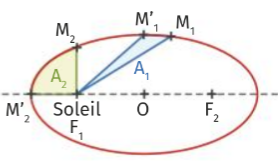
\includegraphics[scale=.5]{Ressources/TSPE_C6_Ex_Fig1.png}
	\end{center}
\end{minipage}

\begin{enumerate}
	\item Justifier la position du Soleil indiquée sur le schéma ci-dessus en cotant la loi de Kepler utilisée.
\textcolor{blue}{L'orbite de Rhéa Sylvia décrit une ellipse autours du Soleil, selon la première loi de Kepler : si l'orbite décrit une ellipse alors l'astre attracteur, ici le Soleil, est positionné à l'un des foyers de l'ellipse. Cela explique la position du Soleil sur le schéma.}
	\item On suppose que les durées de parcours entre les points $M_1$ et $M_1'$, puis $M_2$ et $M_2'$ sont égales. En utilisant une des lois de Kepler, donner la relation existante entre les aires $A_1$ et $A_2$.
	\textcolor{blue}{Selon la deuxième loi de Kepler, pour des durées égales les aires balayées par un objet en orbite autour d'un astre attracteur sont égales, donc $A_1 = A_2$}
\end{enumerate}

\section*{Exercice 2 : Rencontre de la sonde Cassini avec Saturne}
Lors de sa mission d'exploration, la sonde européenne Cassini-Huygens a livré les premiers clichés de Saturne, noté S, de ses anneaux et de ses nombreux satellites dont Titan, noté T, le plus grand, de masse $M$. On considérera que son centre décrit une trajectoire circulaire autour de Saturne.
\begin{enumerate}
	\item Représenter qualitativement sur un schéma Saturne, Titan et la force de gravitation appliquée sur Titan.\\
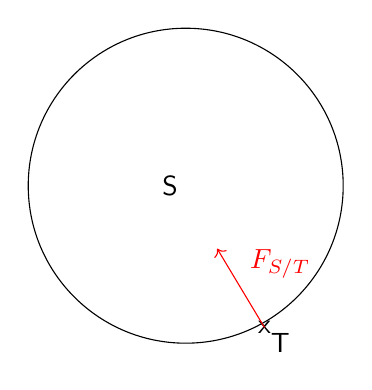
\begin{tikzpicture}
\draw (5,0) circle (2);
\node (S) at (4.8,0) {S};
\node (T) at (6.2,-2) {T};
\node (P) at (6,-1.8) {x};
\draw [->][color=red] (6,-1.8) -- (5.4,-.8);
\node (F)[color=red] at (6.2,-1) {$\vv{F_{S/T}}$};
\end{tikzpicture}
	\item Donner l'expression vectorielle de cette force.\\
\textcolor{blue}{L'expression de la force d'attraction gravitationnelle, placée dans le repère de Frenet donne : $\vv{F_{S/T}} = G \cdot \dfrac{M_S \cdot M}{r_T^2} \cdot \vec{N}$}
	\item Exprimer l'accélération vectorielle de Titan en précisant la loi utilisée. Préciser ses caractéristiques.\\
\textcolor{blue}{L'accélération vectorielle est accessible en appliquant la deuxième loi de Newton à Titan : $\sum \vec{F}= M \cdot \vec{a}$ ce qui donne $\vv{F_{S/T}}= M \cdot \vec{a}$. En remplaçant $\vv{F_{S/T}}$ par l'expression précédente on obtient : $G \cdot \dfrac{M_S \cdot M}{r_T^2} \cdot \vec{N} = M \cdot \vec{a}$ soit en simplifiant : $\vec{a} = G \cdot \dfrac{M_S }{r_T^2} \cdot \vec{N}$\\
Le vecteur accélération aura les caractéristiques suivantes : 
\begin{eqnarray}
	\vec{a} = \left\lbrace
	\begin{array}{l}
	a_T = 0\\
	a_N = G \cdot \dfrac{M_S }{r_T^2}
	\end{array}
	\right\rbrace \nonumber
\end{eqnarray}}
	\item Montrer que le mouvement de Titan est uniforme.\\
\textcolor{blue}{On constate que la composante $a_T$ est nulle, or on sait que $a_T = \dfrac{dv}{dt}=0$ ce qui implique que la vitesse, primitive de l'accélération, est constante sur toute l'orbite. Le mouvement est donc circulaire et uniforme.}
	\item Montrer que l'expression de la vitesse orbitale de Titan autour de Saturne est $v_T = \sqrt{\dfrac{G \cdot M_S}{r_T}}$. Calculer sa valeur.\\
\textcolor{blue}{On sait que $a_N = \dfrac{v^2}{r_T}$ or on a déterminé précédemment que $a_N = G \cdot \dfrac{M_S }{r_T^2}$. En égalant les deux expressions on obtient : 
\begin{eqnarray}
	\dfrac{v^2}{r_T} = G \cdot \dfrac{M_S }{r_T^2}  \nonumber \\
	\leftrightarrow v^2 = G \cdot \dfrac{M_S }{r_T} \nonumber \\
	\leftrightarrow v = \sqrt{G \cdot \dfrac{M_S }{r_T}} \nonumber \\
	\text{AN :} v = \sqrt{6,67\times 10^{-11} \cdot \dfrac{5,69 \times 10^{26} }{1,22 \times 10^{9}}} =\num{5,58e3} \unit{\meter \per \second} \nonumber
\end{eqnarray}}
\end{enumerate}
\textbf{Données :}
\begin{itemize*}
	\item \textbf{Constante de gravitation universelle :} $G$ = \num{6,67e-11}\unit{ \meter \cubed \per \kilo \gram \per \second \squared}
	\item \textbf{Rayon de l'orbite de Titan :} $r_T$ = \num{1,22e6} \unit{\kilo \meter}
	\item \textbf{Rayon de Saturne :} $R_S$ = \num{5,8e4} \unit{\kilo \meter}
	\item \textbf{Masse de Saturne :} $M_S$ = \num{5,69e26} \unit{\kilo \gram}
\end{itemize*}

\section*{Exercice 3 : Alphasat, satellite géostationnaire européen}
Le satellite Alphasat a été mis en orbite géostationnaire par la société Arianespace depuis Kourou en 2013. Il a pour but d'assurer des missions de télécommunications. Il se déplace suivant une trajectoire supposée circulaire de rayon $r$ et possède une masse $m$.
\begin{enumerate}
	\item Expliquer ce qu'est un satellite géostationnaire.\\
\textcolor{blue}{Une orbite géostationnaire est une orbite circulaire dans le plan équatorial de la Terre de période orbitale égale à la période de rotation de la Terre.}
	\item Préciser le référentiel le plus adapté pour étudier le mouvement du satellite, assimilé à un point ponctuel $S$.\\
\textcolor{blue}{Le référentiel le plus adapté à l'étude de ce mouvement est le référentiel géocentrique.}
	\item Dans le repère de Frenet, retrouver l'expression du vecteur accélération $\vec{a_S}$ de $S$ tel que sa valeur est égale à $a_s=G \cdot \dfrac{M_T}{r^2}$.\\
\textcolor{blue}{Dans le repère de Frenet, on peut appliquer la deuxième loi de Newton : $\sum \vec{F}= M \cdot \vec{a}$. Ici la seule force à considérée est la force d'attraction gravitationnelle exercée par la Terre sur le satellite soit : $\vv{F_{S/T}} = G \cdot \dfrac{M_T \cdot m}{r^2} \cdot \vec{N}$. La deuxième loi de Newton donnera donc : $m \cdot \vec{a} = G \cdot \dfrac{M_T \cdot m}{r^2} \cdot \vec{N}$. Donc : $a_S = G \cdot \dfrac{M_T}{r^2}$}
\end{enumerate}



\section*{Exercice 4 : Trajectoire d'une comète}
\begin{minipage}{.5\textwidth}
La trajectoire d'une comète est tracée ci-dessous dans le référentiel héliocentrique. On suppose que les durées  de parcours entre les points $M_1$ et $M_1'$, puis $M_2$ et $M_2'$ sont égales. La comète est soumise à l'attraction gravitationnelle du Soleil. Toute autre attraction est négligeable.\\
\end{minipage}
\begin{minipage}{.5\textwidth}
	\begin{center}
	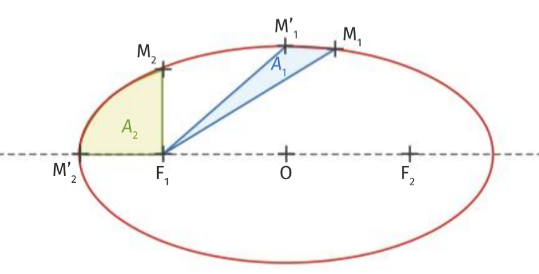
\includegraphics[scale=.5]{Ressources/TSPE_C6_Ex_Fig3.png}
	\end{center}
\end{minipage}
\begin{enumerate}
	\item Après avoir identifié la forme de la trajectoire, préciser ce que représentent les points $F_1$, $F_2$ et $O$.\\
	\textcolor{blue}{La trajectoire de la comète est une ellipse dont les points $F_1$ et $F_2$ sont les foyers et le point $O$ constitue le centre.}
	\item Déterminer sur quel parcours entre $M_1M_1'$ ou $M_2M_2'$ la vitesse de la comète est la plus importante. Expliquer.\\
\textcolor{blue}{La deuxième loi de Kepler nous dit que pour une même durée, l'aire balayée par un objet en orbite elliptique autour d'un astre est égale. On constate donc que pour une même durée, la distance $M_1M_1'$ est plus courte que $M_2M_2'$. La comète sera donc plus rapide pour parcourir la distance $M_2M_2'$.}
	\item Représenter la force d'interaction gravitationnelle exercée sur la comète sur un point de la trajectoire\\
\begin{center}
	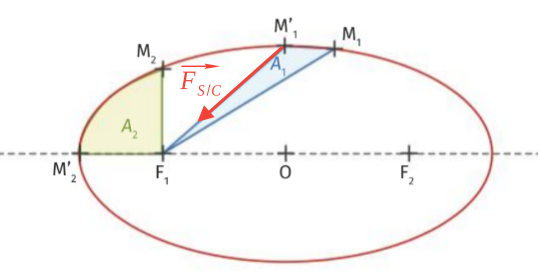
\includegraphics[scale=.5]{Ressources/TSPE_C6_Ex_Fig3bis.png}
	\end{center}
\end{enumerate}



\section*{Exercice 5 : Couchers de soleils dur Tatooine}
\begin{minipage}{.5\textwidth}
Dans la saga \textit{Star Wars}, Tatooine a la particularité d'être en orbite autour de deux étoiles Tatoo 1 et Tatoo 2. Du point de vue de la planète, tout se passe comme si les étoiles n'en faisaient qu'une. On peut estimer que leur distance est légèrement supérieure à 10 millions de kilomètres. En vérité, pour ne pas être inhabitable et expliquer son aspect désertique, une bonne position de Tatooine serait de deux cents millions de kilomètres.
\end{minipage}
\begin{minipage}{.5\textwidth}
\begin{center}
	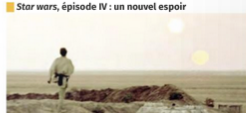
\includegraphics[scale=1]{Ressources/TSPE_C6_Ex_Fig4.png}
\end{center}
\end{minipage}
\begin{enumerate}
	\item En supposant que Tatoo 1 et Tatoo 2 sont à égale distance de Tatooine, montrer, en s'appuyant sur la photo et sur le texte, que la valeur du rayon de chacune des deux étoiles est environ égale à deux millions de kilomètres.
	\item En supposant que les étoiles possèdent la même masse volumique que le Soleil, évaluer leur masse.
\end{enumerate}
On estime pour la suite que la masse des deux étoiles est égale à $M_{tatoo}$ = \num{9,3e31} \unit{\kilo \gram}.
\begin{enumerate}
\setcounter{enumi}{2}
	\item Faire un schéma du système Tatooine-Tatoo$_{1-2}$ et représenter sans soucis d'échelle la force d'attraction gravitationnelle exercée par Tatoo$_{1-2}$ sur Tatooine ainsi que le vecteur accélération de Tatooine.
	\item Montrer que le mouvement, supposé circulaire, de la planète dans ce référentiel est uniforme.
	\item Déterminer la période de révolution de Tatooine. Conclure.
\end{enumerate}
\textbf{Données :}
\begin{itemize*}
	\item \textbf{Rayon :} $R_{Soleil}$ = \num{7,0e5} \unit{\kilo \meter}
	\item \textbf{Masse :} $M_{Soleil}$ = \num{2,0e30} \unit{\kilo \gram}
	\item \textbf{Volume d'une sphère de rayon $r$ :} $V=\dfrac{4}{3}\pi \cdot r^3$
\end{itemize*}
\end{document}